\chapter{序論}
\label{introduction}
本章では本研究の背景と全体の構成について記述する.

\section{背景}
\label{introduction:background}



% \subsection{Data plane}
% \subsubsection{IDC市場の広がり}
% % 単純にIDC事業が伸びていることを言う.


% 近年,ライブ映像配信のようなリアルタイムなサービスに対するニーズが年々高まっている.例えばCisco社の調査\cite{index2017global}によれば,2022年には全てのアプリケーショントラフィックのうちインターネットビデオが有する割合が82%を超え,そのうち17%がライブ映像配信が占めると予想されている.
% リアルタイムな高品質サービスを提供するためには,ユーザーの地理的に近いサービス拠点から配信を行うことが有効であるため,今後IDC・コンテンツ事業者が各地域拠点を介したコンテンツ配信基盤を活用するしていくことが予想される.

% %災害リスクから拠点を増やしたい話
% また,インフラストラクチャに対する災害や地政学的リスクの軽減は,コンテンツ事業者の継続的な事業の成長のためには避けては通れない課題である\cite{alonso2001business}.
% 2011年に発生した東日本大震災以降,国内のIDC事業者やコンテンツ事業者を中心に,関東大都市圏に集中していたサービス拠点への依存性を解消するために,東京圏以外の各地域にサービス拠点を分散する取り組みが活発である\cite{JANOG44_robust}.大阪・名古屋の他の都市圏のIDCは2019年現在満床状態が続いているほか,他の地方拠点都市も含めたIDC建設も並行して行われている. 

% 特に,近年ではVXLAN(Virtual eXtensible Local Area Network)\cite{RFC7348}やSRv6\cite{RFC8402}のような新しいネットワーク仮想化技術の標準化も進み,サービス拠点のマルチテナンシーと柔軟性を両立するネットワークデザインの障壁が低くなってきているため,今後より多くのIDC・コンテンツ事業者のサービス拠点の拡大が続くと想定される.


% \subsubsection{IPv4アドレスの枯渇}
% \label{introduction:background:ipv4_problems}
% 2019年現在,IANA\footnote{Internet Assigned Numbers Authority.インターネットに利用される様々な資源を一元的に管理する組織.\url{https://www.iana.org/}}が保有するIPv4アドレスプールは既に枯渇しており\cite{IANA_allocation},各RIR\footnote{Regional Internet Registry.地域レジストリ.インターネット資源はIANA,地域レジストリ,国別レジストリを介して各自律システムに配分される.}からも2021年頃までには新規割当が行えなくなることが予想されている\cite{potaroo_IPv4}.各RIRが有するアドレスプールの残余量の推移を図\ref{fig:potaroo_IPv4}に示す.

% \begin{figure}
% 	\centering
% 	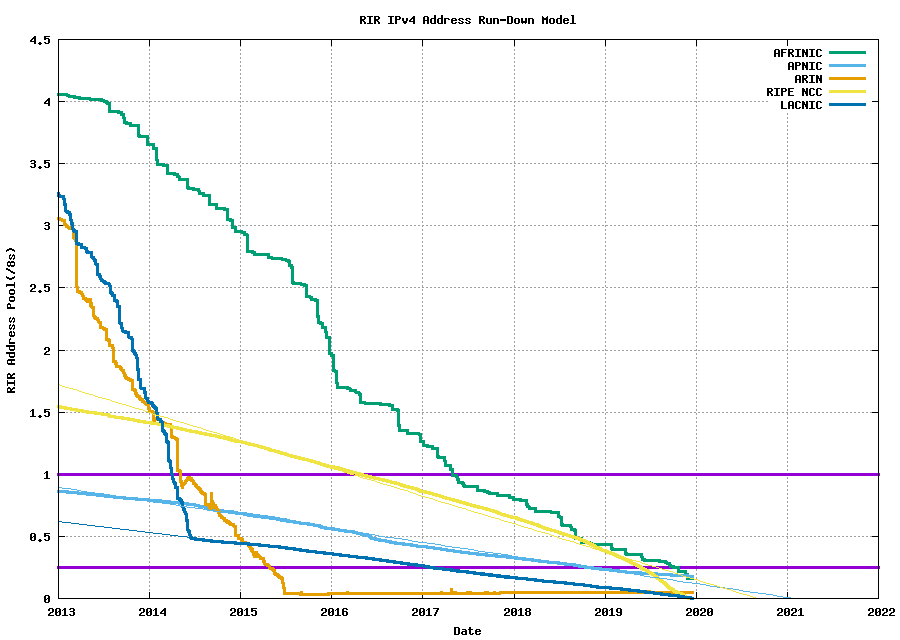
\includegraphics[width=12cm]{img/plotend.png}
% 	\caption{Projection of consumption of Remaining RIR Address Pools. \url{potaroo.net}より引用\cite{potaroo_IPv4}}
% 	\label{fig:potaroo_IPv4}
% \end{figure}
    
% また,近年は民間事業者間アドレス取引も盛んに行われている.一般に新規にIPv4アドレスの割当を受けるためにはこのような民間取引市場を利用する方法が考えられるが,1アドレスあたりの単価は年々上昇傾向にあり\cite{howard2013internet},新規にIPv4ネットワークを構築するためのコストは日々上昇していくことが考えられる.


% \subsubsection{IPv6への移行}
% \label{introduction:background:ipv6_transition}
% 1998年にIPv6標準仕様が策定されて以降\cite{RFC2460},2019年現在までIPv6インターネットとIPv4インターネットの独立した二つのインターネットが並行して存在する状態が続いている.

% 一方で,インターネット技術はIPv6を前提とした設計が行われる段階を迎えている.2016年にはIAB\footnote{Internet Architecture Board. \url{https://www.iab.org/}}により,"IAB Statement on IPv6"が発表され,インターネット標準はIPv6に最適化した標準策定を行う方針が確認されている\cite{IAB_statement}.例えば既にSRv6のような新しい標準はIPv6の拡張ヘッダーを利用した技術として策定が進められており,IPv4を前提とした長期的なネットワーク運用は限界を迎えている.

% \subsubsection{IPv4/IPv6デュアルスタックネットワークの問題}
% \label{introduction:background:dualstack_problems}
% IPv6プロトコルの導入に際し,主に用いられていた手法としてIPv4/IPv6デュアルスタックネットワークが挙げられる\cite{durand2001deploying}.これは,IPv4ネットワークとIPv6ネットワークを同一機器群上に並行して運用する手法であり,企業・一般家庭向けアクセスネットワークを中心に,IPv4/IPv6デュアルスタック環境による整備が進められた.

% 一般的にコンテンツ事業者が運用するIDCでは,主に以下の3つの理由からデュアルスタック環境の導入はデメリットが大きい.

% \begin{itemize}
%     \item \textbf{IPv4アドレスの継続的調達が困難} \\
%     IPv4アドレスをサービスの成長にあわせて継続的に調達していくことは困難である.民間市場の市況に調達コストが左右されるため長期的な見通しが立てにくい.
%     \item \textbf{オペレーションコストの肥大化}\\
% デュアルスタック環境では2つの異なるIPプロトコルを同時に運用する必要があるため、シングルスタック環境と比べて運用コストの上昇が見込まれる\cite{北口善明2017クライアント}.
%     \item \textbf{ネットワーク機器の性能要件の上昇}\\
% デュアルスタック環境では,シングルスタック環境よりも多くの経路をネットワーク機器が保持しなければならないため,より高性能な機器を導入する必要がある.
% \end{itemize}



% \subsection{IPv6シングルスタックネットワーク}
% \label{introduction:background:IPv6-single-stack-network}
% IDC事業者・コンテンツ事業者がビジネスを健全に拡大するためには,IPv6ネットワークのみで機器間を接続したIPv6シングルスタックネットワークの利用が不可欠である.

% IDCのIPv6シングルスタックネットワークには以下のような働きが期待される.


% \subsubsection{IPv4サービスの提供}
% \label{introduction:background:IPv6-single-stack-network:ipv4-service}
% Google社が定常的に行っている調査\cite{Google_IPv6_statistics}によれば,2019年12月現在全世界のインターネットトラフィックの7割程度は依然としてIPv4トラフィックが占めている.
% 将来的にはIPv6トラフィックの割合が徐々に大きくなることが予想されるが,今後しばらくはIPv4クライアントに対してもIPv6クライアントと同等にサービス提供を行っていくことが必要とされる.

% コンテンツ事業者のIPv6シングルスタックネットワークにおいても,何らかの手段を用いてIPv4サービスを継続して提供する機構を備える必要がある.

% \subsubsection{シングルスタック運用によるOPEX/CAPEXの削減}
% 第\ref{introduction:background:dualstack_problems}項で述べたように,IPv4/IPv6デュアルスタックネットワークではオペレーションコストの肥大化が問題視されている.
% IPv6シングルスタックネットワークではIPv4ネットワークを廃止することが出来るため,OPEX\footnote{Operating expense. 運用に掛かる継続的なコスト.}とCAPEX\footnote{Capital expenditure. 設備配備に掛かる初期投資コスト.}の軽減が期待出来る.
% またIPv6アドレスはIPv4アドレスと比較して広大なアドレススペースを有するため,アドレススペースに依存しない柔軟なネットワーク設計が可能になる.

% \subsubsection{IPv4/IPv6デュアルスタックネットワークと同等以上の性能}
% IPv6により提供されるサービスはもちろんのこと,IPv4によるサービスにおいてもIPv4/IPv6デュアルスタックネットワークと同等の耐障害性・サービス品質・サービス容量が保証されることが望ましい.

% とりわけネイティブなIPv4ネットワーク以外の手段を用いて提供されるIPv4サービスの性能の担保が運用課題になると考えられる.




\section{本研究の目的}

本研究では,Layer-4 ロードバランサにおける
% 本研究では,IDC・コンテンツ事業者のネットワークに於いて,IPv6シングルスタックネットワークを基本としながら,IPv4サービスを効率的に提供するための技術の設計・開発を行う.

% 本提案手法ではIPv6シングルスタックネットワークにおけるIPv4サービスの提供手法のうち,アーキテクチャがシンプルで広範な利活用が期待されるSIIT-DC\cite{RFC7755}に着目した.
% SIIT-DCとはIPv6ネットワークとIPv4ネットワークの各境界部に,BR\footnote{Border Relay. IP/ICMP変換アルゴリズム\cite{RFC7915}を実装したIPv4/IPv6トランスレーション機器.}を配備することにより,IPv6ネットワークのみに属するホストで仮想的にIPv4サービスを提供するネットワーク設計を定めたインターネット標準である.SIIT-DCにおいて各BRは静的に定義されたアドレス変換テーブルを利用してネットワークプロトコル変換を行うため,BRを複数配備する場合における変換テーブルの一貫性の確保や冗長性,IDC内の構成変更に対する追従性の面で課題がある.

% 本研究では動的経路アルゴリズムの一つであるBGP\cite{RFC4271}を利用したメッセージングによるアドレス変換テーブルの動的な広告手法を提案し,概念実証用ネットワークを利用した評価実験により,SIIT-DCの課題に対して効果的に作用することを評価する.



\section{本論文の構成}

本論文の構成を以下に示す.

~第\ref{related}章では,IPv6シングルスタックネットワークにおけるIPv4サービス提供手法に関してそれぞれの特徴や利点を紹介し比較する.

~第\ref{issue}章では,IPv4/IPv6プロトコル変換を利用したIPv4サービス提供手法の一つであるSIIT-DCのアーキテクチャと,解決すべき課題について明らかにする.

~第\ref{consideration}章では,SIIT-DCの課題を解決するために考えられる手法について論ずる.

~第\ref{proposal}章では,本研究において提案するダイナミックなアドレス変換テーブル広告手法の要件と構成について記述する.またメッセージングプロトコルとして採用したBGPの技術的利点について述べる.

~第\ref{implementation}章では,本提案手法のBGPメッセージのペイロード設計と第\ref{evaluation}章でも評価実験に用いるPoC(Proof of Concept)の具体的な実装について述べる.

~第\ref{evaluation}章では,第\ref{issue}章で述べた課題に対して,本提案手法が有用であることを検証するための実証実験の概要及び具体的なシナリオについて述べ,結果を考察する.

~第\ref{conclusion}章では,本研究のまとめと本研究の展望について検討する.

%%% Local Variables:
%%% mode: japanese-latex
%%% TeX-master: "../thesis"
%%% End:
